\documentclass[frenchb,DIV=14]{scrartcl}

\usepackage[utf8x]{inputenc}
\usepackage[T1]{fontenc}
\usepackage{lmodern}
\usepackage[binary-units=true]{siunitx}
% Color
% cfr http://en.wikibooks.org/wiki/LaTeX/Colors
\usepackage{color}
\usepackage[usenames,dvipsnames,svgnames,table]{xcolor}
\definecolor{dkgreen}{rgb}{0.25,0.7,0.35}
\definecolor{dkred}{rgb}{0.7,0,0}
\usepackage{graphicx}
\usepackage{url}
\usepackage{tikz}
\usepackage{pgfplots}
\usepackage{microtype}
\usepackage{xspace}

\usepackage{hyperref}
\usepackage{todonotes}
\usepackage{epstopdf}

\usepackage{multirow}
\usepackage{tabularx} % tabular with automatic line-break
\newcolumntype{Y}{>{\centering\arraybackslash}X} % centered column

\newcommand{\matlab}{\textsc{Matlab}}

% Math symbols
\usepackage{amsmath}
\usepackage{amssymb}
\usepackage{amsthm}
\DeclareMathOperator*{\argmin}{arg\,min}
\DeclareMathOperator*{\argmax}{arg\,max}

% Unit vectors
\usepackage{esint}
\usepackage{esvect}
\newcommand{\kmath}{k}
\newcommand{\xunit}{\hat{\imath}}
\newcommand{\yunit}{\hat{\jmath}}
\newcommand{\zunit}{\hat{\kmath}}
\newcommand{\uunit}{\hat{\umath}}

% Elec
\newcommand{\B}{\vec B}
\newcommand{\E}{\vec E}
\newcommand{\EMF}{\mathcal{E}}
\newcommand{\perm}{\varepsilon} % permittivity

\newcommand{\bigoh}{\mathcal{O}}
\newcommand\eqdef{\triangleq}

\DeclareMathOperator{\newdiff}{d} % use \dif instead
\newcommand{\dif}{\newdiff\!}
\newcommand{\fpart}[2]{\frac{\partial #1}{\partial #2}}
\newcommand{\ffpart}[2]{\frac{\partial^2 #1}{\partial #2^2}}
\newcommand{\fdpart}[3]{\frac{\partial^2 #1}{\partial #2\partial #3}}
\newcommand{\fdif}[2]{\frac{\dif #1}{\dif #2}}
\newcommand{\ffdif}[2]{\frac{\dif^2 #1}{\dif #2^2}}
\newcommand{\constant}{\ensuremath{\mathrm{cst}}}
\newcommand{\norm}[1]{\left\lVert#1\right\rVert}

\usepackage{babel}
% Listing
% always put it after babel
% http://tex.stackexchange.com/questions/100717/code-in-lstlisting-breaks-document-compile-error
\usepackage{listings}

% Put caption after babel
\usepackage{caption}
\usepackage{subcaption}

\definecolor{mygreen}{rgb}{0,0.6,0}
\definecolor{mygray}{rgb}{0.5,0.5,0.5}
\definecolor{mymauve}{rgb}{0.58,0,0.82}
\lstset{ %
  language=Matlab,
  backgroundcolor=\color{white},   % choose the background color; you must add \usepackage{color} or \usepackage{xcolor}
  basicstyle=\footnotesize,        % the size of the fonts that are used for the code
  breakatwhitespace=false,         % sets if automatic breaks should only happen at whitespace
  breaklines=true,                 % sets automatic line breaking
  captionpos=b,                    % sets the caption-position to bottom
  commentstyle=\color{mygreen},    % comment style
  deletekeywords={...},            % if you want to delete keywords from the given language
  escapeinside={\%*}{*)},          % if you want to add LaTeX within your code
  extendedchars=true,              % lets you use non-ASCII characters; for 8-bits encodings only, does not work with UTF-8
  frame=single,	                   % adds a frame around the code
  keepspaces=true,                 % keeps spaces in text, useful for keeping indentation of code (possibly needs columns=flexible)
  keywordstyle=\color{blue},       % keyword style
  otherkeywords={*,...},           % if you want to add more keywords to the set
  numbers=left,                    % where to put the line-numbers; possible values are (none, left, right)
  numbersep=5pt,                   % how far the line-numbers are from the code
  numberstyle=\tiny\color{mygray}, % the style that is used for the line-numbers
  rulecolor=\color{black},         % if not set, the frame-color may be changed on line-breaks within not-black text (e.g. comments (green here))
  showspaces=false,                % show spaces everywhere adding particular underscores; it overrides 'showstringspaces'
  showstringspaces=false,          % underline spaces within strings only
  showtabs=false,                  % show tabs within strings adding particular underscores
  stepnumber=1,                    % the step between two line-numbers. If it's 1, each line will be numbered
  stringstyle=\color{mymauve},     % string literal style
  tabsize=2,	                   % sets default tabsize to 2 spaces
  title=\lstname                   % show the filename of files included with \lstinputlisting; also try caption instead of title
}

\KOMAoptions{DIV=last}



\usetikzlibrary{intersections}
\usepgfplotslibrary{fillbetween}
\pgfdeclarelayer{bg}
\pgfsetlayers{bg,main}

\titlehead{}
\subject{LELEC1530}
\title{Séance complémentaire - circuits digitaux}
\subtitle{Solutions}
\author{\small Gaëtan \textsc{Cassiers} \and\small Antoine \textsc{Paris}}
\date{}

\begin{document}
\maketitle

\emph{Cette séance est basée sur la partie "exercices complémentaires" du syllabus d'exercice.}

\section*{Exercice 4 : Circuit combinatoire}
Implémentez et dimensionnez la fonction $X = \overline{ABCD} + E$ en logique domino
et en CMOS sur base de l'inverseur unitaire ($L_{min}=\SI{50}{nm}$, $W_n=\SI{500}{nm}$,
$W_p=\SI{1000}{nm}$). Comparez la surface de silicium nécessaire à l'implémentation en
ne comptant que la surface occupée par les transistors.

\hspace{1cm}\hrule\hspace{1cm}

\subsection*{Implémentation en logique CMOS}
En logique CMOS, une porte logique est constituée d'une partie \emph{pull-up} (en PMOS, car
les PMOS sont bons pour passer des 1) et d'une partie \emph{pull-down} (en NMOS, car les
NMOS sont bons pour passer des 0). La sortie $X$ d'un circuit en logique CMOS peut se
trouver de deux manières :
\begin{enumerate}
	\item En passant par le réseau pull-up : $X = f_u(\bar{A}, \bar{B}, \dots)$ ;
	\item En passant par le réseau pull-down : $X = \overline{f_d(A, B, \dots)}$.
\end{enumerate}
En logique CMOS, on a toujours $f_u(\bar{A}, \bar{B}, \dots) = \overline{f_d(A, B, \dots)}$.
Cela signifie deux choses. Premièrement, la sortie n'est jamais tirée à la fois vers la 
masse et vers $V_{DD}$. Deuxièmement la sortie n'est jamais flottante (elle est toujours
tirée soit vers la masse, soit vers $V_{DD}$). \\

Dans cet exercice, $X = \overline{ABCD} + E$. On constate donc qu'il est impossible
d'écrire $X$ comme une fonction uniquement des compléments $\bar{A}, \bar{B}, \dots$
ou comme le complément d'une fonction des litéraux $A, B, \dots$. On a donc deux
possibilités :
\begin{enumerate}
	\item On peut réecrire $X = \overline{ABCD\bar{E}}$. La fonction logique peut
	donc être implémentée en un seul étage avec une NAND à 5 entrées et un inverseur
	pour obtenir $\bar{E}$ ;
	\item La fonction logique peut être implémentée en plusieurs étages : une NAND
	à 4 entrée pour obtenir $\overline{ABCD}$, suivi d'une NOR et puis d'une NOT pour
	obtenir $X$.
\end{enumerate}

Si le but est d'optimiser la surface de silicium utilisée, la première solution
est légèrement préférable. L'implémentation est donnée à la figure~\ref{fig:ex4-cmos}.

\begin{figure}
	\centering
	\begin{circuitikz}
		\draw
		% 4NAND
		(2.25,2) node[vcc] {$V_{DD}$}
		(0,2) -- (4.5,2)
    	(0,0) to [Tpmos,n=p1] (0,2)
    	(p1.G) node[anchor=east] {$A$}
    	(1.5,0) to [Tpmos, n=p2] (1.5,2)
    	(p2.G) node[anchor=east] {$B$}
    	(3.0,0) to [Tpmos, n=p3] (3.0,2)
    	(p3.G) node[anchor=east] {$C$}
    	(4.5,0) to [Tpmos, n=p4] (4.5,2)
    	(p4.G) node[anchor=east] {$D$}
    	(0,0) -- (6,0)
    	(2.25, -1.5) to [Tnmos, n=n1] (2.25, 0)
    	(n1.G) node[anchor=east] {$A$}
    	(2.25, -3.0) to [Tnmos, n=n2] (2.25, -1.5)
    	(n2.G) node[anchor=east] {$B$}
    	(2.25, -4.5) to [Tnmos, n=n3] (2.25, -3.0)
    	(n3.G) node[anchor=east] {$C$}
    	(2.25, -6) to [Tnmos, n=n4] (2.25, -4.5)
    	(n4.G) node[anchor=east] {$D$}
    	(2.25, -6) node[ground] {}
    	
    	% 2NOR
    	(8,2) node[vcc] {$V_{DD}$}
    	(8, 0.5) to [Tpmos, n=p5] (8,2)
    	(6,0) -- (6,1.25) -- (p5.G)
    	(8, -1) to [Tpmos, n=p6] (8,0.5)
    	(p6.G) node[anchor=east] {$E$}
    	(7.25,-2.5) to [Tnmos,n=n5] (7.25,-1)
    	(8.75,-2.5) to [Tnmos, n=n6] (8.75,-1)
    	(n6.G) node[anchor=east] {$E$}
    	(6,0) -- (6,-1.75) -- (n5.G)
    	(7.25, -1) -- (8.75, -1)
    	(7.25, -2.5) -- (8.75, -2.5)
    	(8, -2.5) node[ground] {}
    	
    	% NOT
    	(10, -1) node[not port](mynot){}
    	(8.75, -1) -- (mynot.in)
    	(mynot.out) node[anchor=west] {$X$}
    	;
	\end{circuitikz}
	\caption{Implémentation CMOS de $X = \overline{ABCD} + E$.}
	\label{fig:ex4-cmos}
\end{figure}

\paragraph{Dimensionnement}
On dimensionne ensuite comme d'habitude par rapport à l'inverseur unitaire.
\begin{enumerate}
	\item PMOS de la 4-NAND : $20/1$ ;
	\item NMOS de la 4-NAND : $40/1$ ;
	\item PMOS de la 2-NOR : $40/1$ ;
	\item NMOS de la 2-NOR : $10/1$. 
\end{enumerate}
On trouve donc que la surface totate est donnée par $370L_{min}^2$ (l'autre solution
proposée donne une surface de $380L_{min}^2$).

\subsection*{Implémentation en logique domino}
Une implémentation possible est donnée à la figure~\ref{fig:ex4-domino}

\begin{figure}
	\centering
	\begin{circuitikz}
		\draw
		% 4NAND
		(2.25,2) node[vcc] {$V_{DD}$}
		(0,2) -- (4.5,2)
    	(0,0) to [Tpmos,n=p1] (0,2)
    	(p1.G) node[anchor=east] {$A$}
    	(1.5,0) to [Tpmos, n=p2] (1.5,2)
    	(p2.G) node[anchor=east] {$B$}
    	(3.0,0) to [Tpmos, n=p3] (3.0,2)
    	(p3.G) node[anchor=east] {$C$}
    	(4.5,0) to [Tpmos, n=p4] (4.5,2)
    	(p4.G) node[anchor=east] {$D$}
    	(0,0) -- (6,0)
    	(2.25, -1.5) to [Tnmos, n=n1] (2.25, 0)
    	(n1.G) node[anchor=east] {$A$}
    	(2.25, -3.0) to [Tnmos, n=n2] (2.25, -1.5)
    	(n2.G) node[anchor=east] {$B$}
    	(2.25, -4.5) to [Tnmos, n=n3] (2.25, -3.0)
    	(n3.G) node[anchor=east] {$C$}
    	(2.25, -6) to [Tnmos, n=n4] (2.25, -4.5)
    	(n4.G) node[anchor=east] {$D$}
    	(2.25, -6) node[ground] {}
    	
    	% 2NOR
    	(8,2) node[vcc] {$V_{DD}$}
    	(8, 0.5) to [Tpmos, n=p5] (8,2)
    	(6,0) -- (6,1.25) -- (p5.G)
    	(8, -1) to [Tpmos, n=p6] (8,0.5)
    	(p6.G) node[anchor=east] {$E$}
    	(7.25,-2.5) to [Tnmos,n=n5] (7.25,-1)
    	(8.75,-2.5) to [Tnmos, n=n6] (8.75,-1)
    	(n6.G) node[anchor=east] {$E$}
    	(6,0) -- (6,-1.75) -- (n5.G)
    	(7.25, -1) -- (8.75, -1)
    	(7.25, -2.5) -- (8.75, -2.5)
    	(8, -2.5) node[ground] {}
    	
    	% NOT
    	(10, -1) node[not port](mynot){}
    	(8.75, -1) -- (mynot.in)
    	(mynot.out) node[anchor=west] {$X$}
    	;
	\end{circuitikz}
	\caption{Implémentation CMOS de $X = \overline{ABCD} + E$.}
	\label{fig:ex4-cmos}
\end{figure}

\paragraph{Dimensionnement}

\section*{Exercice 5: Logique dynamique}
On considère le circuit en logique dynamique de la figure~\ref{fig9-2} dans une technologie
\SI{50}{nm}. Voici les paramètres technologiques :
\begin{center} 
	$\begin{array}{l l l l}
		L_{min} = \SI{50}{nm} & C_{ox} = 62.5\cdot WL\text{aF} 
		& R_N= 34/W k\Omega
		& R_P= 68/W k\Omega \\ 
	\end{array}$
\end{center}

\begin{figure}[]
   \centering
   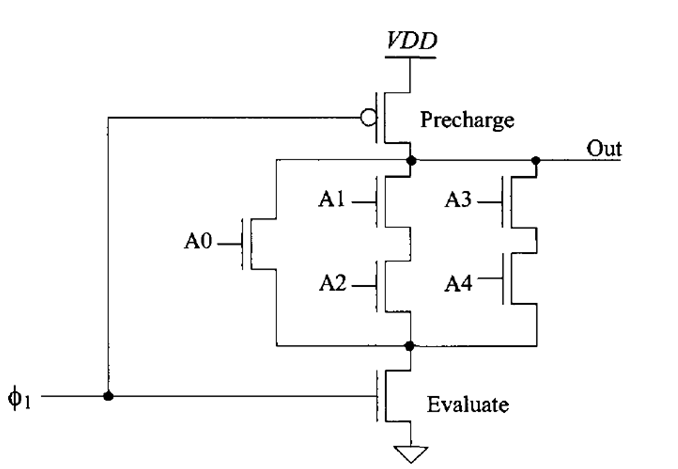
\includegraphics[width=14cm]{figures/fig9-2.png}
   \caption{Exercice 5, logique dynamique.}
   \label{fig9-2}
\end{figure}

\begin{enumerate}
	\item Quelle est la fonction logique implémentée ?
	\item Dimensionnez la porte par rapport à l'inverseur unitaire ($L_{min}=\SI{50}{nm}$,
	$W_n=\SI{500}{nm}$ et $W_p=\SI{1000}{nm}$).
	\item Calculez le délai $t_{PHL}$ à 50\% lorsque $A_0$=1 et $A_{1->4}$=0 si la sortie
	est connectée à une capacité de charge $C_L$ de \SI{50}{\femto\farad}.
\end{enumerate}

\hspace{1cm}\hrule\hspace{1cm}

\paragraph{Fonction logique implémentée}
La fonction logique implémentée est donnée par
\[ \text{Out} = \overline{A_0 + A_1A_2 + A_3A_4}.\]

\paragraph{Dimensionnement}
On dimensionne comme d'habitude par rapport à l'inverseur unitaire.
\begin{itemize}
	\item PMOS de pré-charge : $20/1$ ;
	\item NMOS $A_{1\to4}$ et NMOS d'évaluation : $30/1$ ;
	\item NMOS $A_0$ : $15/1$. 
\end{itemize}

\paragraph{Délai}
Si $A_{1\to4} = 0$, la sortie se décharge uniquement à travers $A_0$
et le NMOS d'évaluation. On a donc une décharge à travers deux transistors
en série. On sait que le temps de déchage $t_{PHL}$ à travers $N$
transistors \emph{identiques} en séries peut être estimé par
\[ t_{PHL} = 0.35R_nC_{oxn}N^2 + 0.7NR_nC_{load}. \]
Le problème ici est que le transistor $A_0$ est différent du transistor
d'évaluation vu le dimensionnement effectué au point précédent.
Une approche serait par exemple d'utiliser la moyenne de $R_n$ et $C_{oxn}$
sur ces deux transistors. Cela donne
\[ R_{n,avg} = \frac{1}{2} \cdot \left(\frac{34}{15} + \frac{34}{30}\right)\SI{}{\kilo\ohm}
= \SI{1.7}{\kilo\ohm} \]
et
\[ C_{oxn,avg} = \frac{1}{2} \cdot \left(62.5\cdot 15 + 62.5\cdot 30)\right)\SI{}{\atto\farad}
= \SI{2.9125}{\femto\farad}. \]
Quand à $C_{load}$, on a
\[ C_{load} = C_L + C_{outp} + (\frac{C_{oxn,avg}}{2} + 2\frac{C_{outn}}{2})
|| \frac{C_{oxn,avg}}{2}. \]

\section*{Exercice 6: full adder}

On considère un additionneur sur 1 bit présenté à la figure~\ref{fig9-3} dans
une technologie \SI{50}{nm}. Voici les paramètres technologiques :
\begin{align*}
    L_{min} &= \SI{50}{nm} &
    C_{ox} &= \SI{62.5}{aF}\cdot W\cdot L &
    R_N&=\SI{34}{k\ohm}/W &
    R_P&=\SI{68}{k\ohm}/W 
\end{align*}

\begin{figure}
	\centering
	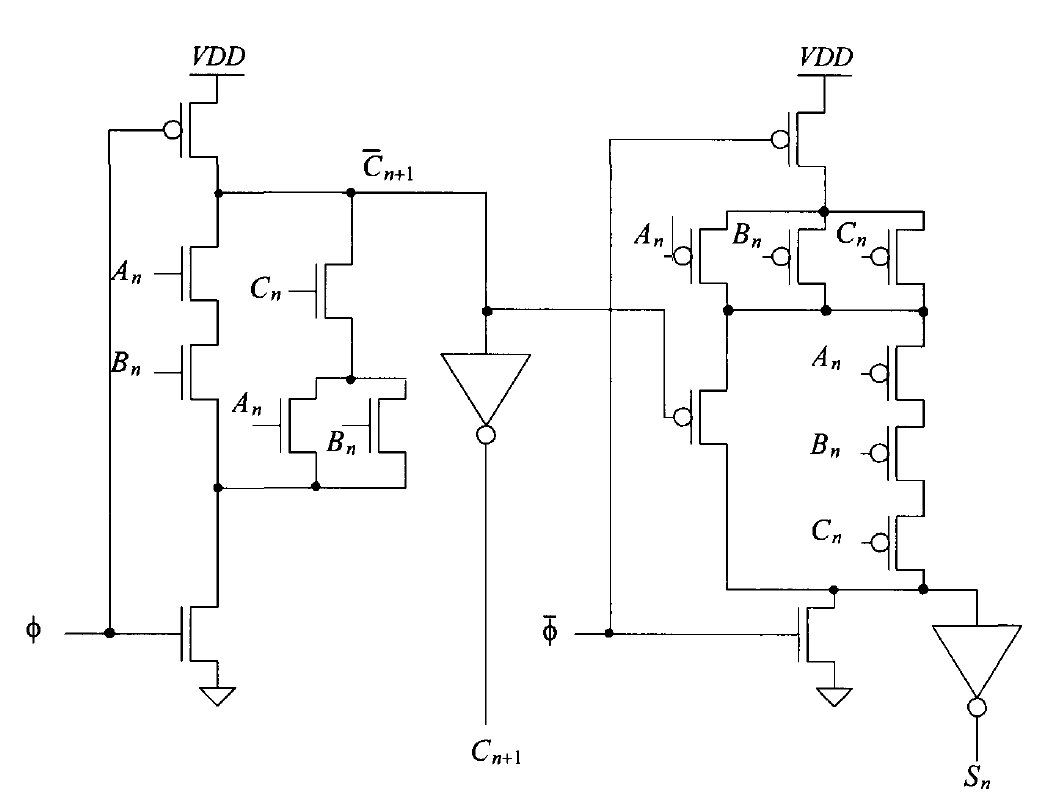
\includegraphics[width=13cm]{figures/fig9-3.png}
	\caption{Exercice 6, full adder.}
	\label{fig9-3}
\end{figure}

\begin{enumerate}
	\item Décrivez le type de logique utilisé dans la Figure \ref{fig9-3}.
	Donnez la fonctionnalité logique de chacune des deux portes sous forme d'une
	table de vérité ainsi que la fonctionnalité logique globale.
	\item Dimensionnez les deux portes logique sur base de l'inverseur
    unitaire ($L_{min}=\SI{50}{nm}$, $W_{n}=\SI{500}{nm}$, $W_{p}=\SI{1000}{nm}$).
	\item Implémentez un additionneur prenant en entrée des mots de 2 bits sur
	base de l'additionneur sur 1 bit de la Figure \ref{fig9-3}.
	\item En considérant un signal d'horologe avec un \emph{duty-cycle} de 50\%,
	quelle est la fréquence maximale de fonctionnement de l'additionneur 2 bits ?
	Quelle est la fréquence maximale si l'architecture implémente une addition sur
	2 mots de 32 bits ?
\end{enumerate}

\hspace{1cm}\hrule

\subsection*{1.}

Logique domino NP (Zipper logic).

\paragraph{Équations logiques}
$C_{n+1} = A_n B_n + C_n (A_n + B_n)$
\begin{align*}
    S_n &= \overline{(\overline{A_n} + \overline{B_n} + \overline{C_n})(C_{n+1} + \overline{A_n}\cdot\overline{B_n}\cdot\overline{C_n})} \\
    &=  \overline{\overline{A_n}+\overline{B_n}+\overline{C_n}} + \overline{C_{n+1} + \overline{A_n}\cdot\overline{B_n}\cdot\overline{C_n}} \\
    &= A_n B_n C_n + \overline{C_{n+1}}(A_n+B_n+C_n)
\end{align*}

\paragraph{Table de vérité}

\begin{center}
    \begin{tabular}{ccc|cc}
        $A_n$&$B_n$&$C_n$&$C_{n+1}$&$S_n$\\
        \hline
        0&0&0&0&0\\
        0&0&1&0&1\\
        0&1&0&0&1\\
        0&1&1&1&0\\
        1&0&0&0&1\\
        1&0&1&1&0\\
        1&1&0&1&0\\
        1&1&1&1&1
    \end{tabular}
\end{center}

\subsection*{2.}

Largeur de transistors (relative à la largeur du transistor correspondant
dans l'inverseur unitaire.

Calcul du \emph{carry} (circuit de gauche):
\begin{itemize}
    \item tous les NMOS: 3
    \item PMOS: 1
\end{itemize}

Calcul de la somme (circuit de droite):
\begin{itemize}
    \item NMOS: 1
    \item PMOS phi: 5
    \item PMOS An, Bn, Cn: 5
    \item PMOS $C_{n+1}$: 3
\end{itemize}

\subsection*{3.}

Utiliser deux full adders 1 bit ($FA_0$ et $FA_1$), connecter le 
\emph{carry-out} ($C_1$) du premier adder au \emph{carry-in} du deuxième. 

\subsection*{4.}

\paragraph{Calcul du délai}

On considère le délai pour un additionneur 1 bit.
Pour un additionneur, on peut considérer 3 délais:
\begin{itemize}
    \item Délai pour le calcul de $\overline{C_{n+1}}$: $t_0$
    \item Délai pour le calcul de $C_{n+1}$ (à partir de $\overline{C_{n+1}}$: $t_1$
    \item Délai pour le calcul de $\overline{S_n}$ (à partir de $\overline{C_{n+1}}$: $t_2$): $t_2$
    \item Délai pour le calcul de $S_n$ (à partur de $\overline{S_n}$): $t_3$
\end{itemize}

Pour la suite, on pose $C_{ox} = \SI{62.5}{aF}$

\subparagraph{Calcul de $t_0$}
Dans le pire cas, chaine de 3 NMOS de largeur 3.
Capacité du noeud $\overline{C_{n+1}}$:
\begin{itemize}
\item Sortie des NMOS: $3/2 C_{ox}$
\item PMOS (de precharge): $C_{ox}$
\item Entrée de l'inverseur: $9/2 C_{ox}$
\item Entrée du PMOS du circuit de la somme: $9 C_{ox}$
\end{itemize}

Capacité totale: $C_{out0} = 16 C_{ox}$.

On a donc
\[t_0 = (0.35\cdot 3^2 C_{ox} + 0.7 C_{out0})\SI{34}{k\ohm} = \SI{30.5}{ps}\]

\subparagraph{Calcul de $t_1$}
Capacité du noeud de sortie $C_{n+1}$: on considère que le carry-out est
connécté au carry-in d'un full adder.
\begin{itemize}
\item Capacité de sortie de l'inverseur $3C_{ox}$
\item NMOS: $9/2 C_{ox}$
\item PMOS: $(6 + 15/2) C_{ox}$
\end{itemize}

Capacité totale: $C_{out1} = 39/2 C_{ox}$.

On a donc
\[t_1 = 0.7 \cdot \SI{34}{k\ohm} C_{out1} = \SI{29.0}{ps}\]

\subparagraph{Calcul de $t_2$}
Dans le pire cas, chaine de 5 PMOS de largeur 5.
Capacité du noeud $\overline{S_n}$:
\begin{itemize}
\item NMOS: $C_{ox}/2$
\item PMOS ($\overline{C_{n+1}}$): $3C_{ox}$
\item PMOS ($C_n$): $5C_{ox}$
\item Entrée de l'inverseur: $9/2 C_{ox}$
\end{itemize}
Capacité totale: $C_{out2} = 13 C_{ox}$

On a donc
\[t_2 = (0.35\cdot 5^2\cdot 2 C_{ox} + 0.7 C_{out2})\SI{34}{k\ohm} = \SI{56.5}{ps}\]

\subparagraph{Calcul de $t_3$}
Sortie d'un inverseur:
\[t_3 = 0.7 \cdot 3 \cdot C_{ox} \SI{34}{k\ohm} = \SI{4.5}{ps}\]

\subparagraph{Délai total}
Au total, le délai pour un additionneur de 2 bits est
\[t_{FA2} = t_0 + t_1 + t_0 + t_2 + t_3 = \SI{151}{ps}\]

\paragraph{Fréquence maximale}
Comme seulement la moitié de le période d'horloge est disponible pour
effectuer les calculs (l'autre moitié est utilisée pour le \emph{prefetch}),
la période d'horloge minimale est \SI{302}{ps}. La fréquence maximale est
donc \SI{3.31}{GHz}.

\paragraph{Additionneur de 32 bits}
Le délai est
\[t_{F32} = 31 (t_0 + t_1) + t_0 + t_2 + t_3 = \SI{1.94}{ns},\]
donc la période d'horloge minimale est de \SI{3.87}{ns}, donc la
fréquence maximale est \SI{258}{MHz}.
\end{document}

